\documentclass{beamer}
\usepackage[utf8]{inputenc}
\usepackage{color}
\usepackage{fancyvrb}
\usepackage{listings}
\usetheme{Berlin}
\setbeamerfont{caption}{size=\footnotesize}

\title{Plateforme pour l'analyse technique en Finance}
\subtitle{Soutenance PFE}
\author{CHAUGNY Céline, POINTIN Damien}
\institute{Génie Mathématique | INSA Rouen}

\begin{document}
\lstset{
keywordstyle=\color[rgb]{0,0,1},
commentstyle=\color[rgb]{0.133,0.545,0.133},
stringstyle=\color[rgb]{0.627,0.126,0.941},
}
    \beamertemplatenavigationsymbolsempty

    \begin{frame}
        \titlepage{}
    \end{frame}

    \section*{Sommaire}
        \begin{frame}
            \begin{columns}[t]
  				\begin{column}{5cm}
  					\tableofcontents[sections={1-4},  hideothersubsections]
  				\end{column}
  				\begin{column}{5cm}
  				\tableofcontents[sections={5-9}, hideothersubsections]
  				\end{column}
  			\end{columns}
        \end{frame}

    \section{Introduction}
        \subsection{ }
            
\begin{frame}
    \frametitle{Introduction}    		
    \begin{block}{But du projet}
	Réaliser un programme pour mettre en place une plateforme permettant la gestion d'un portefeuille. Mise en place d'un jeu dans lequel les investisseurs peuvent acheter de vrais actifs de issus de la bourse.
    \end{block}

    \begin{block}{Phases du projet}
	\begin{enumerate}
	 \item Récupérer et stocker certaines données réelles de la bourse.
	 \item Traiter les donner et les analyser avec des outils financiers.
	 \item Permettre à l'utilisateur d'avoir des indicateurs sur ses actifs.
	\end{enumerate}

    \end{block}

\end{frame}

    \section{Technologies utilisées}
         \subsection{Dynamic Web Project} % celine
         	\begin{frame}
            \begin{columns}[t]
  				\begin{column}{5cm}
  					\tableofcontents[sections={1-4}, sectionstyle=show/shaded,subsectionstyle=show/shaded/hide ]
  				\end{column}
  				\begin{column}{5cm}
  				\tableofcontents[sections={5-9}, sectionstyle=show/shaded,subsectionstyle=show/shaded/hide ]
  				\end{column}
  			\end{columns}
        \end{frame}  
	        \begin{frame}
    \frametitle{Architecture Modèle-Vue-Contrôleur}
    \begin{columns}
  		\begin{column}{5cm}
  		\begin{alertblock}{Vue}
  			Interface Homme-Machine
  		\end{alertblock}
  		\begin{exampleblock}{Contrôleur}
  			Lien entre Modèle et Vue
  		\end{exampleblock}
  		\begin{block}{Modèle}
  			Coeur du programme
  		\end{block}
  		\end{column}
  		
  		\begin{column}{5cm}
  			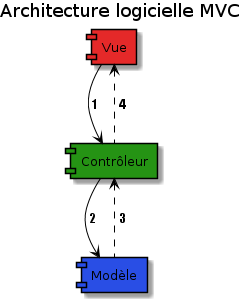
\includegraphics[scale=0.5]{images/MVC.png}
  		\end{column}
  	\end{columns}
\end{frame}

\begin{frame}
    \frametitle{Environnement Java EE sous Eclipse}
    	  \begin{figure}[H]
      \center
      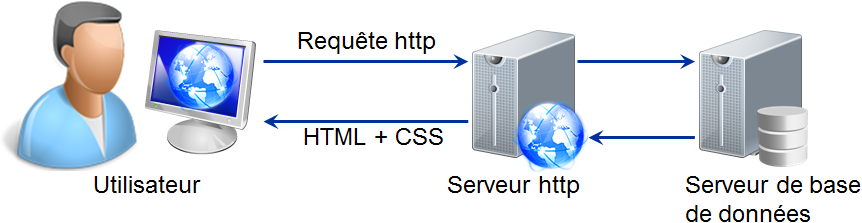
\includegraphics[scale=0.3]{images/protocoleHTTP.png}
      \caption{Application web - Protocole HTTP}
      \end{figure}

	\begin{block}{IDE Eclipse}
		\begin{itemize}
			\item Gratuit, libre, puissant
			\item Auto-complétion, génération automatique de fonction
			\item Visualisation de la hiérarchie
		\end{itemize}
	\end{block}
\end{frame}

\begin{frame}
    \frametitle{Servlet}
    	  \begin{figure}[H]
      \center
      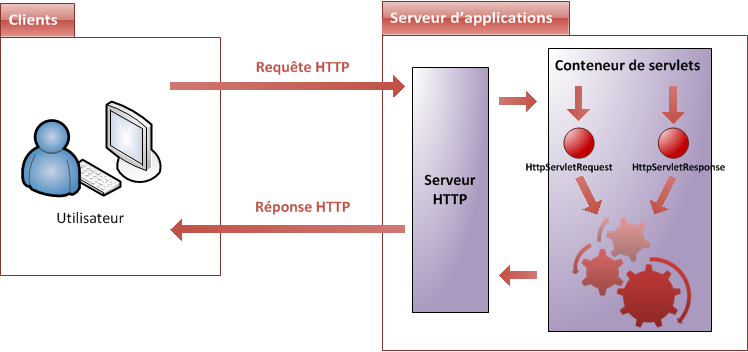
\includegraphics[scale=0.24]{images/serveurclient.png}
      \end{figure}

	\begin{block}{Configuration des servlets}
		\begin{itemize}
			\item Méthode doGet() et doPost()
			\item Configuration dans web.xml
			\item Apache Tomcat 8.0
		\end{itemize}
	\end{block}
\end{frame}


\begin{frame}[fragile]
    \frametitle{Java Server Pages}
    	  
	\begin{block}{JSP}
		\begin{itemize}
			\item Utilisés pour nos pages web dynamiques
			\item Langage : XML, HTML, Javascript, Java, CSS, ...
		\end{itemize}
	\end{block}
	\begin{block}{Java server page Standard Tag Library}
		\begin{itemize}
			\item Tags prédéfinis
			\item \begin{lstlisting}[language=HTML, basicstyle=\scriptsize] 
<%@ taglib uri="http://java.sun.com/jstl/core" 
prefix="c" %>
<c:out value="Bonjour" />
\end{lstlisting}	  
		\end{itemize}	
			
	\end{block}
\end{frame}

\begin{frame}
    \frametitle{Hiérarchie MVC du projet}
    \begin{columns}
  		\begin{column}{3cm}
  		  	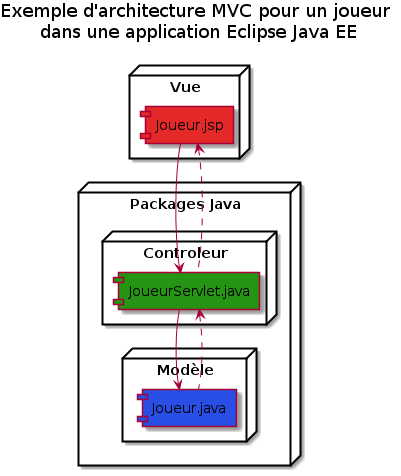
\includegraphics[scale=0.28]{images/exempleMVC.png}

  		\end{column}
  		  		\begin{column}{0.3cm}
  		  		\end{column}

  		\begin{column}{7cm}
  			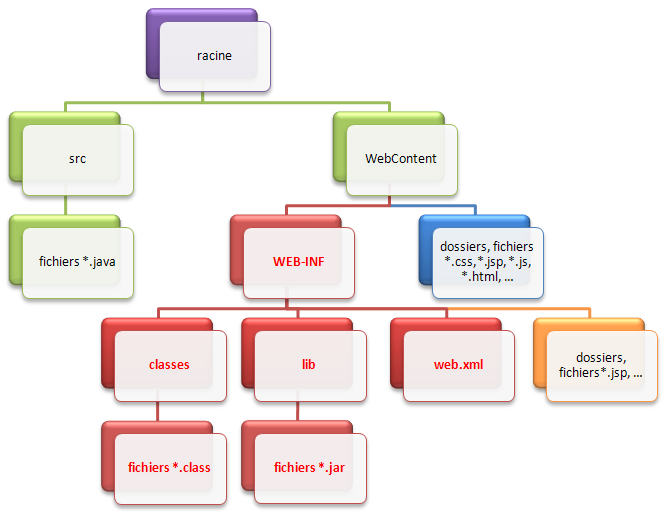
\includegraphics[scale=0.3]{images/schemaProjetDynamic.png}
  		\end{column}
  	\end{columns}
\end{frame}

	     \subsection{Base de données} % nous deux
	        \begin{frame}
            \begin{columns}[t]
  				\begin{column}{5cm}
  					\tableofcontents[sections={1-4}, sectionstyle=show/shaded,subsectionstyle=show/shaded/hide ]
  				\end{column}
  				\begin{column}{5cm}
  				\tableofcontents[sections={5-9}, sectionstyle=show/shaded,subsectionstyle=show/shaded/hide ]
  				\end{column}
  			\end{columns}
        \end{frame}  
	        \begin{frame}
    \frametitle{MySQL -Driver JDBC}
    \begin{block}{MySQL}
    	\begin{itemize}
    		\item Système de gestion de bases de données relationnelles
    		\item Libre, gratuit, open-source
    	\end{itemize}
    \end{block}
     \begin{block}{Driver Java DataBase Connectivity }
     	\begin{columns}
  				\begin{column}{5cm}
  					\begin{itemize}
  						\item Connexion/Déconnexion
  						\item Requête : Statement 
  						\item Résultat : ResulSet
  					\end{itemize}
  				\end{column}
  				\begin{column}{5cm}
  				      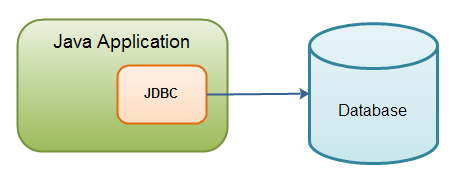
\includegraphics[scale=0.4]{images/jdbc.png}
  				\end{column}
  			\end{columns}

    \end{block}

\end{frame}

\begin{frame}
    \frametitle{Modèle DAO - Principe général}
    \begin{block}{Data Access Object}
    		\begin{itemize}
    			\item Isoler les méthodes concernant le stockage et l'accès aux données
    			\item Création d'une couche supplémentaire :
    		\end{itemize}
    		\center
    		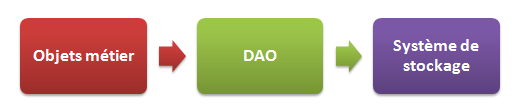
\includegraphics[scale=0.5]{images/dao1.png}
	\end{block}

\end{frame}

\begin{frame}
    \frametitle{Modèle DAO - Mise en place}
     	\begin{columns}
  				\begin{column}{4cm}
  				\begin{block}{Couche DAO}
  				
  					\begin{itemize}
  						\item Méthodes CRUD
  						\item Gestion Exception
  						\item Fabrique 
  						\item Mapping objet-relationnel
  					\end{itemize}
  				\end{block}

  				\end{column}
  				\begin{column}{7cm}
  				      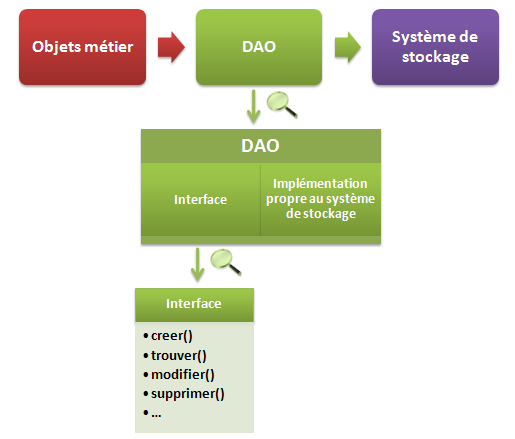
\includegraphics[scale=0.4]{images/dao2.png}
  				\end{column}
  			\end{columns}

\end{frame}    
	    \subsection{Yahoo! Finance} % Damien
	        \begin{frame}
            \begin{columns}[t]
  				\begin{column}{5cm}
  					\tableofcontents[sections={1-4}, sectionstyle=show/shaded,subsectionstyle=show/shaded/hide ]
  				\end{column}
  				\begin{column}{5cm}
  				\tableofcontents[sections={5-9}, sectionstyle=show/shaded,subsectionstyle=show/shaded/hide ]
  				\end{column}
  			\end{columns}
        \end{frame}  
	        \begin{frame}
    \frametitle{Site Yahoo! Finance}
    
    	   \begin{figure}[H]
      \center
      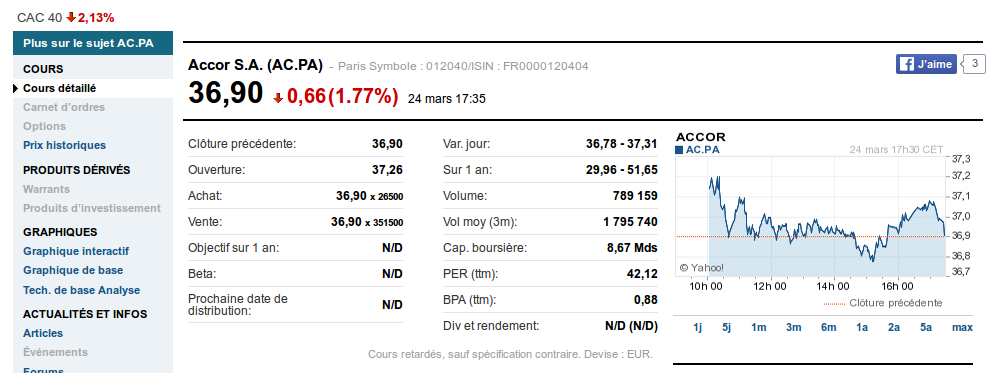
\includegraphics[scale=0.30]{images/yahoo.png}
      \caption{Visualisation du site Yahoo! Finance pour l'action ACCOR S.A}
      \end{figure}
    	   
\end{frame}

\begin{frame}[fragile]
    \frametitle{Principe du téléchargement}
    \begin{block}{Code JAVA}
  \begin{lstlisting}[language=JAVA, basicstyle=\scriptsize] 
String url="http://real-chart.finance.yahoo.com/table.csv?"+
	"s="+code  
	+"&a="+debut.get(Calendar.MONTH) 
	+"&b="+debut.get(Calendar.DAY_OF_MONTH) 
	+"&c="+debut.get(Calendar.YEAR) 
	+"&d="+fin.get(Calendar.MONTH)
	+"&e="+fin.get(Calendar.DAY_OF_MONTH)
	+"&f="+fin.get(Calendar.YEAR)
	+"&g=d" 
	+"&ignore=.csv"; 
\end{lstlisting}	  
	\end{block}

\end{frame}

	    \subsection{API Google Chart} % celine
	        \begin{frame}
            \begin{columns}[t]
  				\begin{column}{5cm}
  					\tableofcontents[sections={1-4}, sectionstyle=show/shaded,subsectionstyle=show/shaded/hide ]
  				\end{column}
  				\begin{column}{5cm}
  				\tableofcontents[sections={5-9}, sectionstyle=show/shaded,subsectionstyle=show/shaded/hide ]
  				\end{column}
  			\end{columns}
        \end{frame}  
	        \begin{frame}
    \frametitle{Présentation de l'API}
    \begin{center}
	      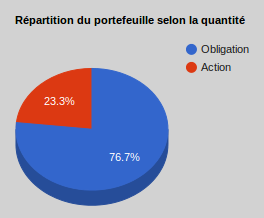
\includegraphics[scale=0.395]{images/google2.png}
	      \hskip1em
	      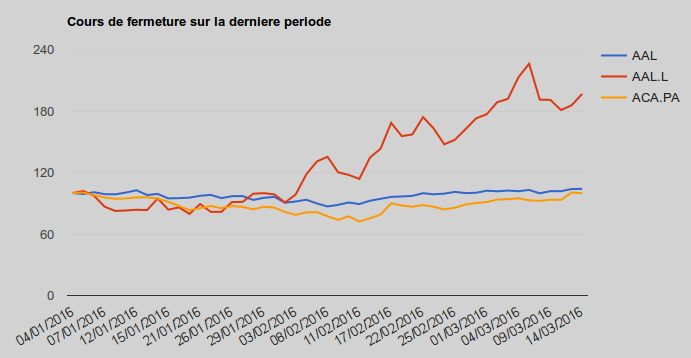
\includegraphics[scale=0.24]{images/google1.png}
    \end{center}
    \begin{block}{Avantages de l'API}
    	\begin{itemize}
    		\item Graphes intéractifs
    		\item Directement dans la JSP avec JavaScript
    	\end{itemize}
    \end{block}
\end{frame}

\begin{frame} [fragile]
    \frametitle{Présentation de l'API}
    \begin{enumerate}
     \item Charger la librairie :
\begin{lstlisting}[language=HTML, basicstyle=\scriptsize] 
<script type="text/javascript"
src="https://www.gstatic.com/charts/loader.js"></script>
<script type="text/javascript">
google.charts.load('current', {packages: ['corechart']});
google.charts.setOnLoadCallback(drawChart);
</script>
\end{lstlisting}	
     \item Préparer les données : créer une DataTable.
\begin{lstlisting}[language=HTML, basicstyle=\scriptsize] 
var data = new google.visualization.DataTable();
data.addColumn('string', 'Actifs');
data.addColumn('number', 'Quantite');
data.addRows([ ['Obligation', 76.7],['Action', 23.3]]);
\end{lstlisting}
 
    \end{enumerate}
\end{frame}

\begin{frame} [fragile]
    \frametitle{Présentation de l'API}
    \begin{enumerate}
     \setcounter{enumi}{2}
     \item Personnaliser le graphe : titre, dimensions, couleurs,...
\begin{lstlisting}[language=JAVA, basicstyle=\scriptsize]      
var options = { title: 'Repartition portefeuille'};
\end{lstlisting}    
     \item Dessiner le graphe : choix du type de graphe.
\begin{lstlisting}[language=JAVA, basicstyle=\scriptsize]      
var chart = new google.visualization.PieChart(
  document.getElementById('camembert'));
chart.draw(data, options);
\end{lstlisting}    
     \item Afficher le graphe : choisir l'emplacement dans la page HTML.
\begin{lstlisting}[language=HTML, basicstyle=\scriptsize]      
<div id="camembert"></div>
\end{lstlisting}    
    \end{enumerate}
\end{frame}       
        	
     \section{Théorie Finance}
        \subsection{Produits financiers} % celine
	        \begin{frame}
            \begin{columns}[t]
  				\begin{column}{5cm}
  					\tableofcontents[sections={1-4}, sectionstyle=show/shaded,subsectionstyle=show/shaded/hide ]
  				\end{column}
  				\begin{column}{5cm}
  				\tableofcontents[sections={5-9}, sectionstyle=show/shaded,subsectionstyle=show/shaded/hide ]
  				\end{column}
  			\end{columns}
        \end{frame}          
	        
\begin{frame}
    \frametitle{Action - Indice}
    \begin{block}{Action}
  	\begin{itemize}
  		\item Partie du capital de la société émettrice
  		\item Prix suit le jeu de l'offre et de la demande
  		\item Droits politiques et droit financiers
  	\end{itemize}
  	\end{block}
  	\pause	
	 \begin{block}{Indice}
  	\begin{itemize}
  		\item Panier d'actions reflétant un marché ou un secteur
  		\item Moyenne pondérée des actifs
  		\item CAC40, SBF120, Dow Jones, Nasdaq, ...
  	\end{itemize}
  	\end{block}
\end{frame}

\begin{frame}
    \frametitle{Obligation}
    \begin{block}{Caractéristiques}
    		\begin{itemize}
    			\item Dette de l'émetteur à moyen ou long terme
    			\item Emprunteur/ Créancier
    			\item Etat (emprunt d'état ou obligation souveraine) ou entreprise (obligation du secteur public et corporative)
    			\item Notation pour mesurer le risque
    			\item Obligation convertible
    		\end{itemize}
	\end{block}  
\end{frame}


	    \subsection{Indicateurs techniques} % Damien
	        \begin{frame}
            \begin{columns}[t]
  				\begin{column}{5cm}
  					\tableofcontents[sections={1-4}, sectionstyle=show/shaded,subsectionstyle=show/shaded/hide ]
  				\end{column}
  				\begin{column}{5cm}
  				\tableofcontents[sections={5-9}, sectionstyle=show/shaded,subsectionstyle=show/shaded/hide ]
  				\end{column}
  			\end{columns}
        \end{frame}  
	        
\begin{frame}
    \frametitle{indicateur}
  

\end{frame}  
		\subsection{Gestion Portefeuille} % celine
	        \begin{frame}
            \begin{columns}[t]
  				\begin{column}{5cm}
  					\tableofcontents[sections={1-4}, sectionstyle=show/shaded,subsectionstyle=show/shaded/hide ]
  				\end{column}
  				\begin{column}{5cm}
  				\tableofcontents[sections={5-9}, sectionstyle=show/shaded,subsectionstyle=show/shaded/hide ]
  				\end{column}
  			\end{columns}
        \end{frame}  
	        
\begin{frame}
    \frametitle{Présentation}
    \begin{block}{Définitions}
	\begin{itemize}
	\item \textbf{Gestion de portefeuille :}
	      \begin{itemize}
	      \item Gérer des capitaux sous certaines contraintes
	      \item Choisir une stratégie d'investissement
	      \end{itemize}
	\item \textbf{Différents risques :}
	      \begin{itemize}
	      \item Financiers : marché, crédit, liquidité
	      \item Non financiers : modèle, perte extrême
	      \end{itemize}
	\item \textbf{Profils de rique :}
	      \begin{itemize}
	      \item Risk adverse
	      \item Risk neutral
	      \item Risk lovers/seekers
	      \end{itemize}
	\end{itemize}
    \end{block}


\end{frame}

\begin{frame}
    \frametitle{Actifs risqués}
	  \begin{figure}
	      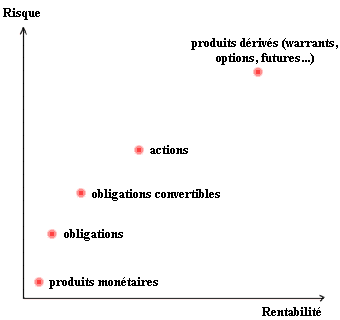
\includegraphics[scale=0.5]{images/actifsRisques.png}   
	  \end{figure}   
\end{frame}


\begin{frame}
    \frametitle{Diversification} 
      \begin{block}{Intérêts}
	\begin{enumerate}
	  \begin{columns}
	    \begin{column}{4cm}
	      \item Eviter les catastrophes
	    \end{column}
	    \begin{column}{4cm}
	      \item Réduire le risque	   
	    \end{column}
	  \end{columns}
	\end{enumerate}
      \end{block}
      \begin{figure}
	  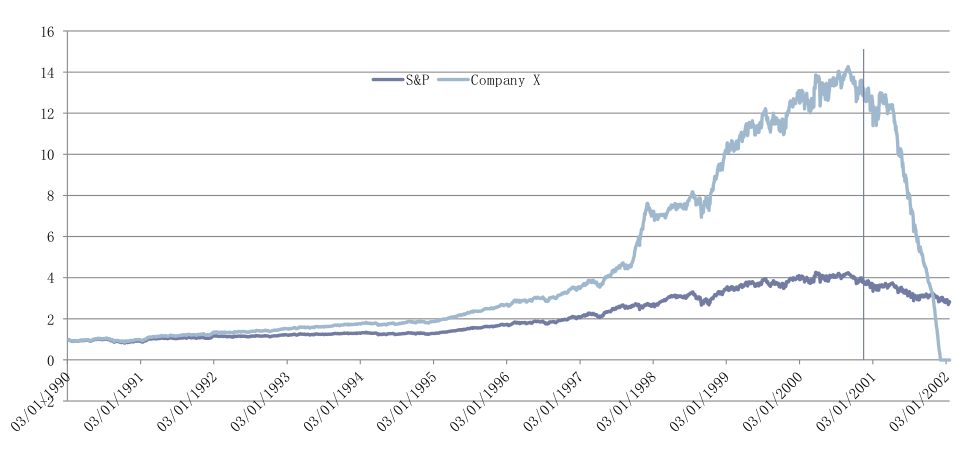
\includegraphics[scale=0.2]{images/exempleChuteEntreprise.png}   
	  \caption{Exemple d'un portefeuille à un actif (courbe bleu ciel)}
      \end{figure}  
\end{frame}



\begin{frame}
    \frametitle{Le rendement} 
    \begin{block}{Rendement d'un actif}
	\begin{itemize}
	 \item Arithmétique :  $R_{i} = \frac{1}{T} \sum_{t=1}^T R_{i,t}$
	 \item Géométrique :  $ R_{i} = \sqrt[T]{\prod_{k=1}^{T}(1+R_{i,k})}-1$
	\end{itemize}
    \end{block}
    \begin{block}{Rendement d'un portefeuille}
	On suppose que l'on a $N$ actifs et on note $w_i$ leur poids respectifs, tels que $\sum_{i=1}^{N}w_i =1$.\\
	Le rendement du portefeuille se calcule ainsi :	$R_P = \sum_{i=1}^{N}w_iR_i$.
    \end{block}
\end{frame}

\begin{frame}
    \frametitle{Le risque} 
    \begin{block}{Risque d'un actif}
	\begin{itemize}
	 \item Variance :  $Var_i = \frac{\sum_{t=1}^T (R_{i,t}-E(R_{i}))^2}{T} $
	 \item Ecart-type :  $ \sigma_i = \sqrt{(Var_i)}$
	\end{itemize}
    \end{block}
    \begin{block}{Risque d'un portefeuille}
	\[\sigma_P^2 = \sum_{i,j=1}^{N}w_iw_jcov(i,j) = \sum_{i=1}^{N}w_i^2Var_i +  \sum_{i,j=1}^{N}w_iw_j\rho_{i,j}\sigma_i\sigma_j\]
    \end{block}
\end{frame}

\begin{frame}
    \frametitle{Optimisation d'un portefeuille} 
    \begin{columns}
      \begin{column}{4.5cm}
	  \begin{block}{Définition}
	      \begin{itemize}
		\item Diversifier selon son profil de risque
		\item Optimiser le couple (rendement, risque)
	      \end{itemize}
	  \end{block}
      \end{column}
      \begin{column}{5.5cm}
	  \begin{figure}
	      \center
	      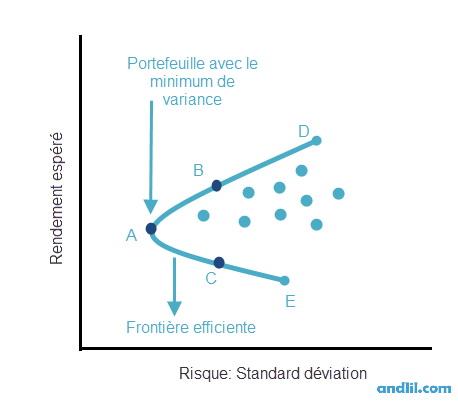
\includegraphics[scale=0.35]{images/frontiereEfficiente.png}   
	      \caption{Frontière efficiente - Problème de Markowitz}
	  \end{figure} 
      \end{column}
    \end{columns}
\end{frame}

\begin{frame}
    \frametitle{Ajout d'un actif sans risque} 
      \begin{figure}
	  \center
	  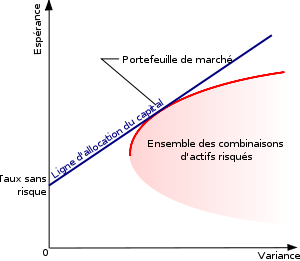
\includegraphics[scale=0.5]{images/cal.png}   
	  \caption{La CAL (Capital Allocation Line)}
      \end{figure} 
\end{frame}

 
	    \subsection{Cadre du projet} % ?
	        \begin{frame}
            \begin{columns}[t]
  				\begin{column}{5cm}
  					\tableofcontents[sections={1-4}, sectionstyle=show/shaded,subsectionstyle=show/shaded/hide ]
  				\end{column}
  				\begin{column}{5cm}
  				\tableofcontents[sections={5-9}, sectionstyle=show/shaded,subsectionstyle=show/shaded/hide ]
  				\end{column}
  			\end{columns}
        \end{frame}  
	        
\begin{frame}
    \frametitle{Le broker (courtier)}
      \begin{block}{Définition}
	   \textbf{Broker :} c'est l'intermédiaire d'une ou des opérations financières entre deux parties. Dans le cadre de notre projet, il est l'intermédiaire entre la bourse et les investisseurs (joueurs).
      \end{block}

      \begin{figure}
	  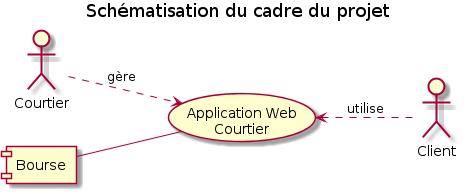
\includegraphics[scale=0.4]{images/schemaProjet.png}
      \end{figure}


\end{frame}
    
	        
	        
	 \section{Modélisation}
        \subsection{Cas d'utilisation}
	        \begin{frame}
            \begin{columns}[t]
  				\begin{column}{5cm}
  					\tableofcontents[sections={1-4}, sectionstyle=show/shaded,subsectionstyle=show/shaded/hide ]
  				\end{column}
  				\begin{column}{5cm}
  				\tableofcontents[sections={5-9}, sectionstyle=show/shaded,subsectionstyle=show/shaded/hide ]
  				\end{column}
  			\end{columns}
        \end{frame}  
	        \begin{frame}
	\begin{figure}
	    	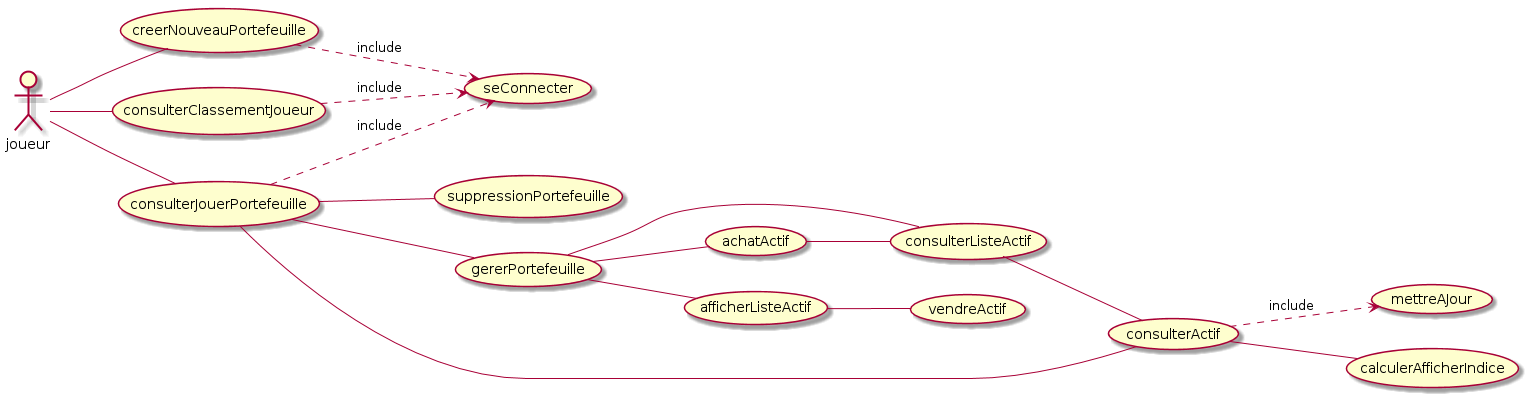
\includegraphics[scale=0.22]{images/CasDutilisationGeneral.png}

	\end{figure}
\end{frame}
	    \subsection{Diagramme classe}
	        \begin{frame}
            \begin{columns}[t]
  				\begin{column}{5cm}
  					\tableofcontents[sections={1-4}, sectionstyle=show/shaded,subsectionstyle=show/shaded/hide ]
  				\end{column}
  				\begin{column}{5cm}
  				\tableofcontents[sections={5-9}, sectionstyle=show/shaded,subsectionstyle=show/shaded/hide ]
  				\end{column}
  			\end{columns}
        \end{frame}  
	        \begin{frame}
    \frametitle{Diagramme Classe Général}
    \begin{figure}
        	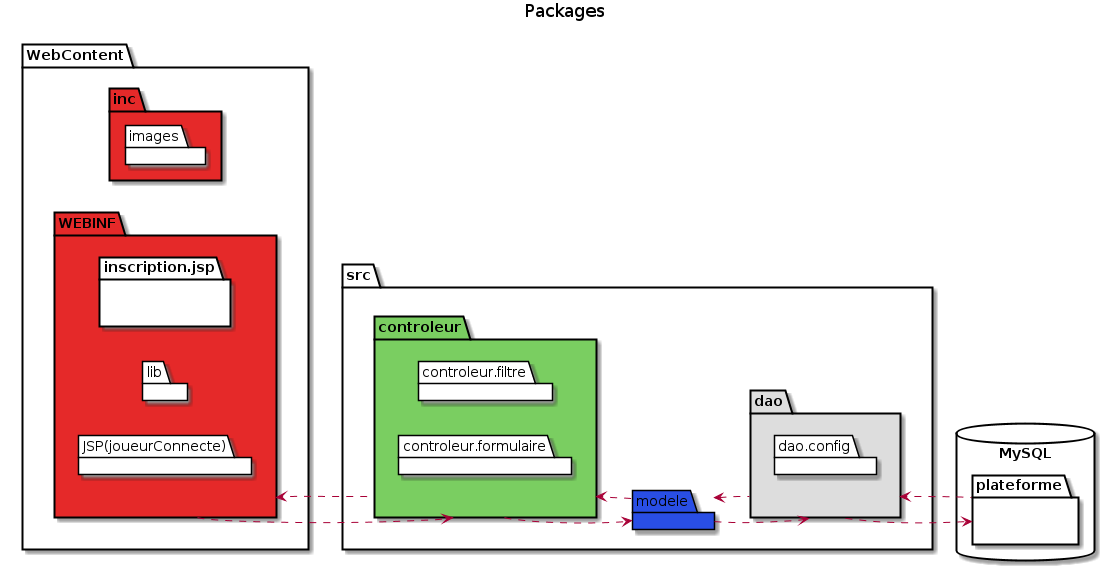
\includegraphics[scale=0.25]{images/packages.png}

    \end{figure}
\end{frame}

\begin{frame}
    \frametitle{Diagramme Classe DAO}
    \begin{figure}
    

    	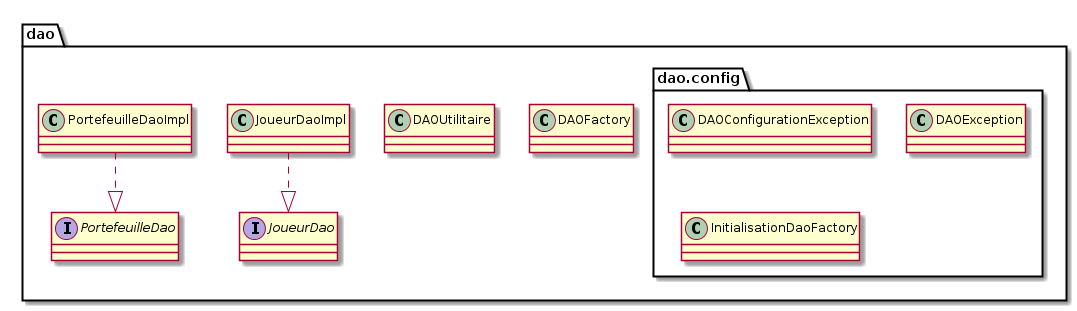
\includegraphics[scale=0.30]{images/packageDAO.png}
    	\end{figure}
\end{frame}

\begin{frame}
    \frametitle{Diagramme Classe Controleur}
    \begin{figure}

    	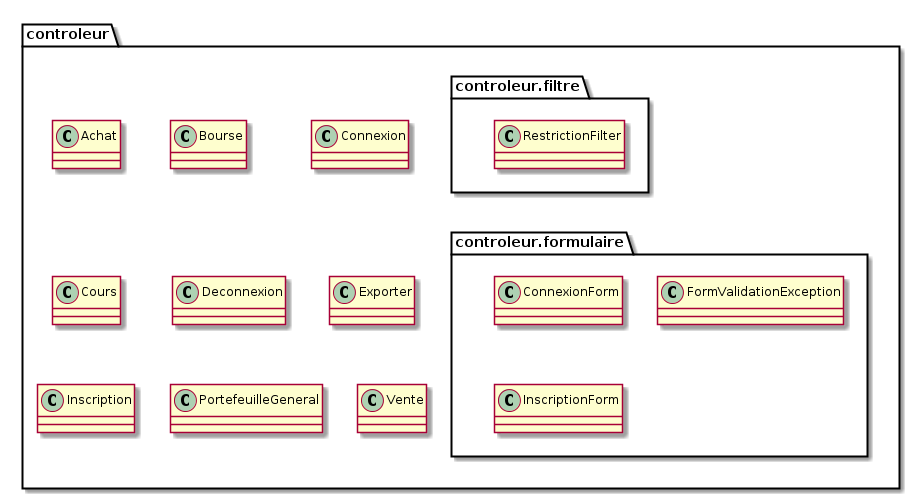
\includegraphics[scale=0.30]{images/packageControleur.png}
    	    	\end{figure}

\end{frame}

\begin{frame}
    \frametitle{Diagramme Classe Modele}
        \begin{figure}

    	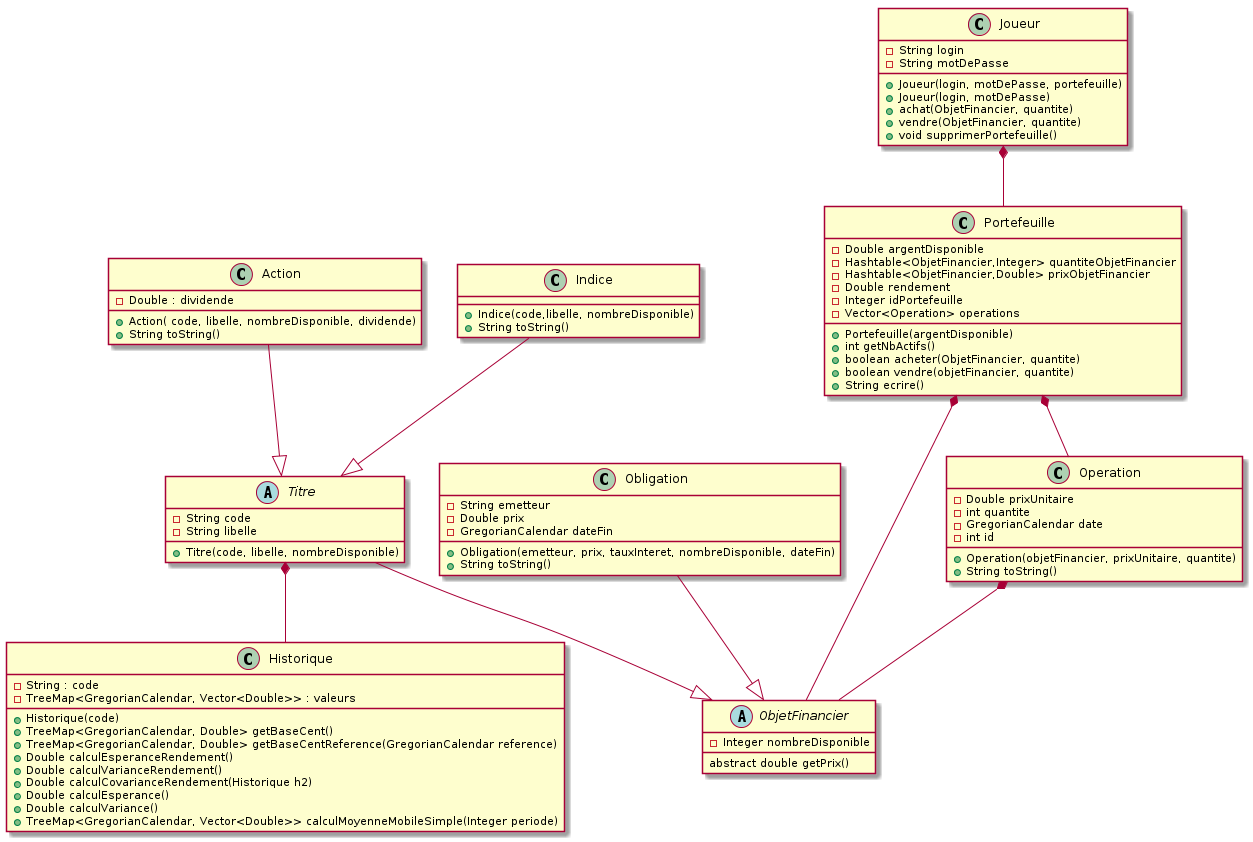
\includegraphics[scale=0.20]{images/DiagrammeClasseFinalModele.png}
    	    	\end{figure}

\end{frame}

\begin{frame}
    \frametitle{Diagramme Architecture WebContent}

    \begin{figure}
    	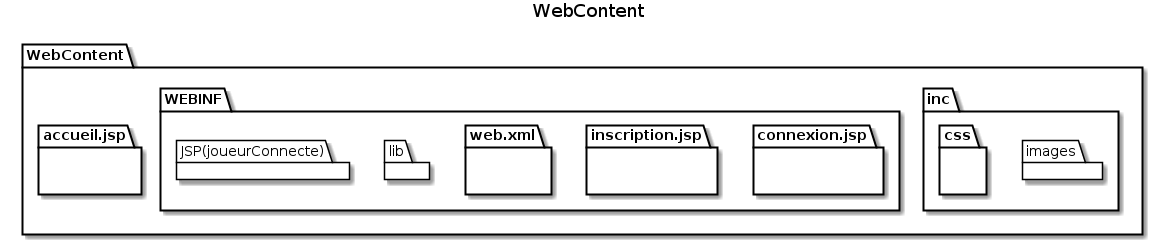
\includegraphics[scale=0.25]{images/packagesWebContent.png}
    	    	\end{figure}

\end{frame}    
		\subsection{Diagramme séquence}
	        \begin{frame}
            \begin{columns}[t]
  				\begin{column}{5cm}
  					\tableofcontents[sections={1-4}, sectionstyle=show/shaded,subsectionstyle=show/shaded/hide ]
  				\end{column}
  				\begin{column}{5cm}
  				\tableofcontents[sections={5-9}, sectionstyle=show/shaded,subsectionstyle=show/shaded/hide ]
  				\end{column}
  			\end{columns}
        \end{frame}  
	        \begin{frame}
    \frametitle{Diagramme Séquence Inscription}
    \begin{figure}
		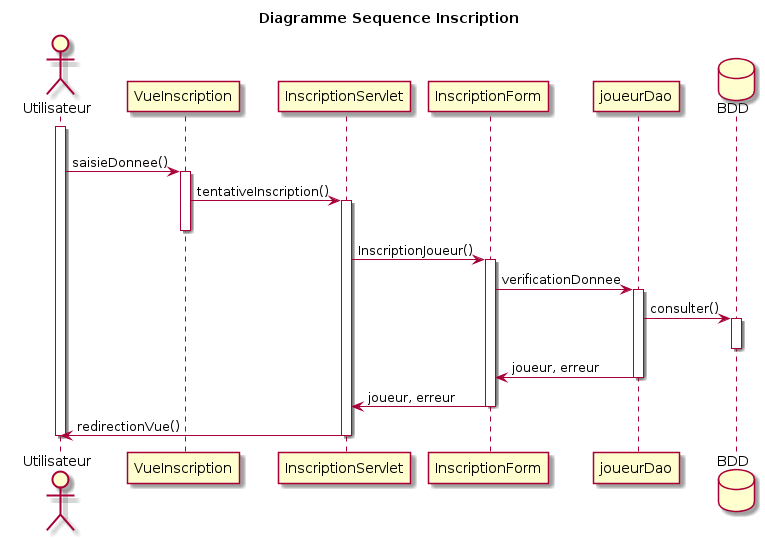
\includegraphics[scale=0.3]{images/DiagrammeSequenceInscription.png}
	\end{figure}

\end{frame}

\begin{frame}
    \frametitle{Diagramme Séquence Connexion}
    \begin{figure}
		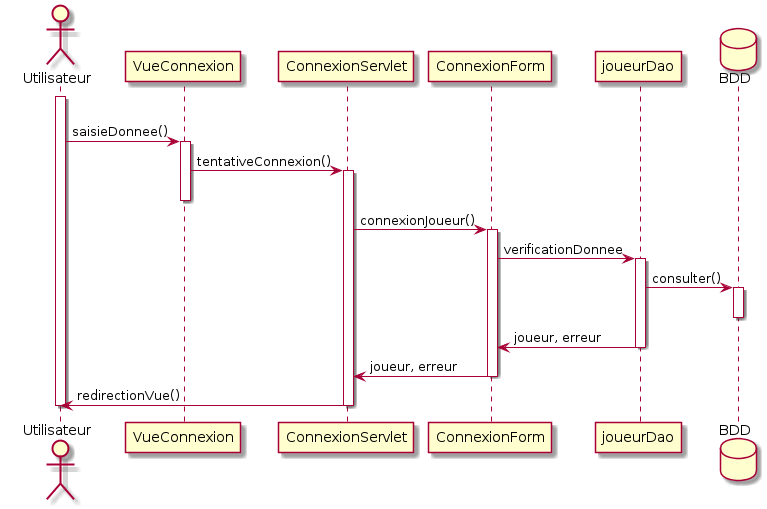
\includegraphics[scale=0.3]{images/DiagrammeSequenceConnexion.png}
	\end{figure}

\end{frame}

\begin{frame}
    \frametitle{Diagramme Séquence Achat Actif}
    \begin{figure}
		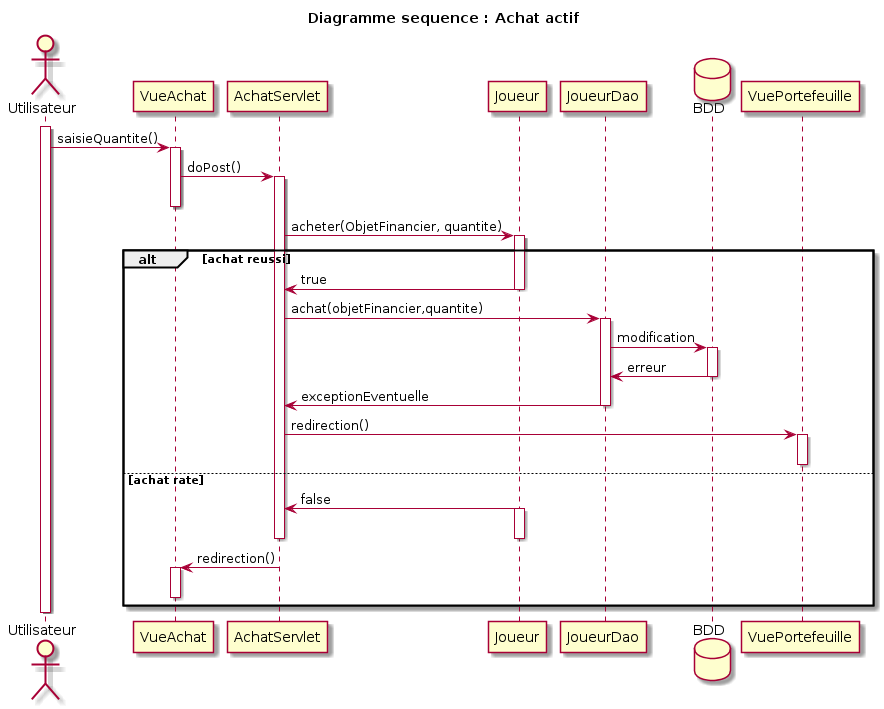
\includegraphics[scale=0.23]{images/DiagrammeSequenceAchatActif.png}
	\end{figure}

\end{frame}

\begin{frame}
    \frametitle{Diagramme Séquence Achat Actif (Zoom modele)}
    \begin{figure}
		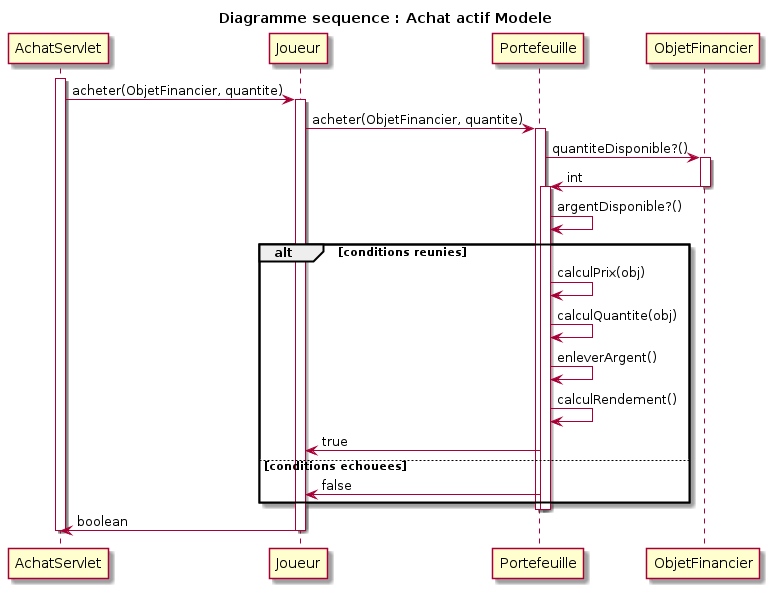
\includegraphics[scale=0.28]{images/DiagrammeSequenceAchatActifModele.png}
	\end{figure}

\end{frame}

\begin{frame}
    \frametitle{Diagramme Séquence Vente Actif}
    \begin{figure}
		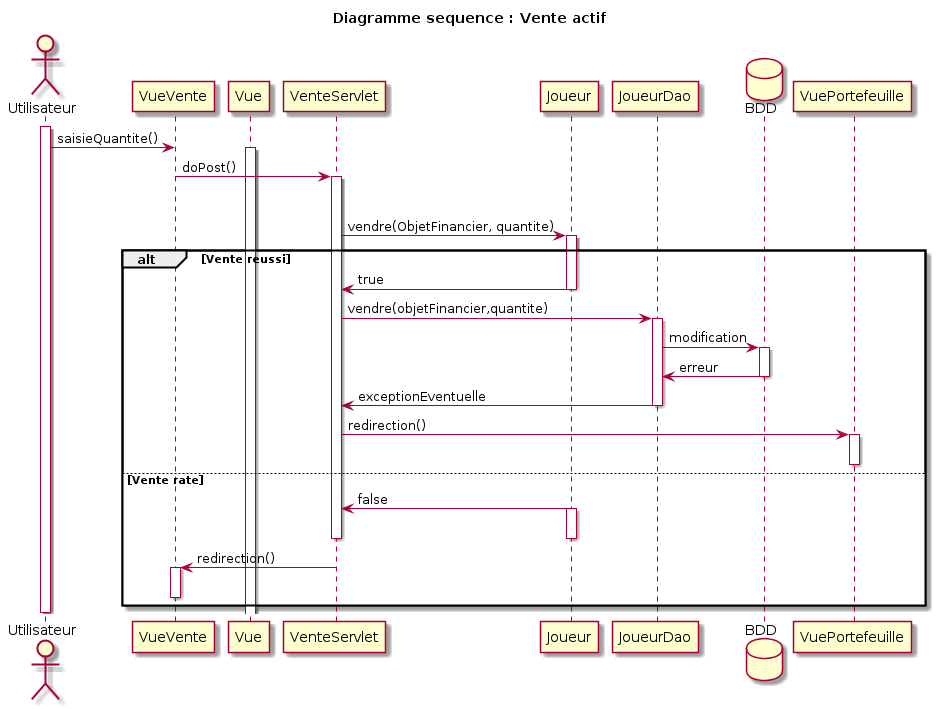
\includegraphics[scale=0.23]{images/DiagrammeSequenceVenteActif.png}
	\end{figure}

\end{frame}

\begin{frame}
    \frametitle{Diagramme Séquence Supprimer Portefeuille}
    \begin{figure}
		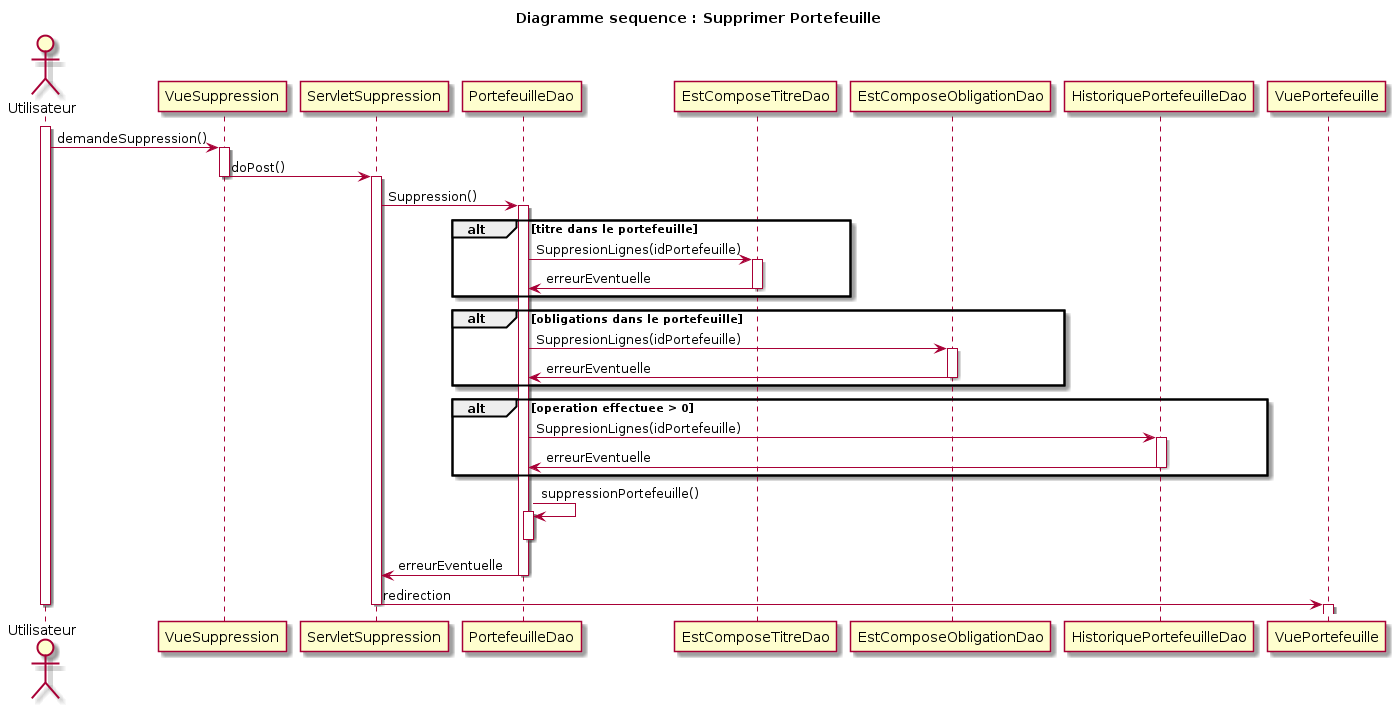
\includegraphics[scale=0.22]{images/DiagrammeSequenceSupprimerPortefeuille.png}
	\end{figure}

\end{frame}
	    \subsection{Base de données}
	        \begin{frame}
            \begin{columns}[t]
  				\begin{column}{5cm}
  					\tableofcontents[sections={1-4}, sectionstyle=show/shaded,subsectionstyle=show/shaded/hide ]
  				\end{column}
  				\begin{column}{5cm}
  				\tableofcontents[sections={5-9}, sectionstyle=show/shaded,subsectionstyle=show/shaded/hide ]
  				\end{column}
  			\end{columns}
        \end{frame}  
	        \begin{frame}
    \frametitle{Schema Entite-Association}
    \begin{figure}
		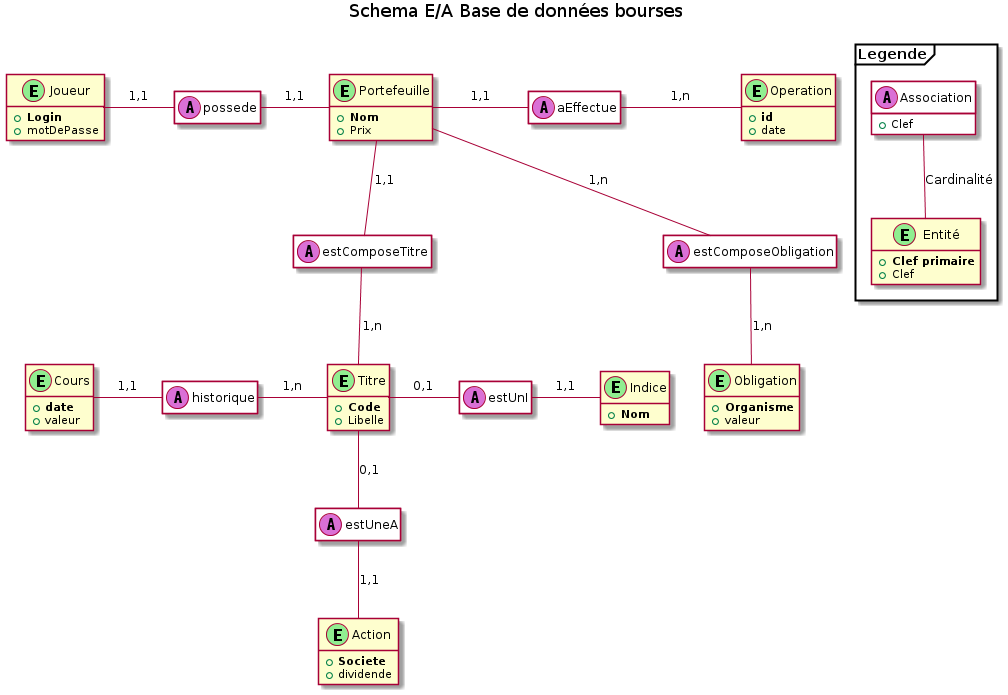
\includegraphics[scale=0.23]{images/DiagrammeEntiteAssociation.png}
	\end{figure}

\end{frame}
	    \subsection{Modélisation de la bourse et portefeuille}
	        \begin{frame}
            \begin{columns}[t]
  				\begin{column}{5cm}
  					\tableofcontents[sections={1-4}, sectionstyle=show/shaded,subsectionstyle=show/shaded/hide ]
  				\end{column}
  				\begin{column}{5cm}
  				\tableofcontents[sections={5-9}, sectionstyle=show/shaded,subsectionstyle=show/shaded/hide ]
  				\end{column}
  			\end{columns}
        \end{frame}  
	        
\begin{frame}
    \frametitle{portefeuille}
  

\end{frame}
    
    \section{Travail de groupe}
        \subsection{Répartition} 
	        \begin{frame}
            \begin{columns}[t]
  				\begin{column}{5cm}
  					\tableofcontents[sections={1-4}, sectionstyle=show/shaded,subsectionstyle=show/shaded/hide ]
  				\end{column}
  				\begin{column}{5cm}
  				\tableofcontents[sections={5-9}, sectionstyle=show/shaded,subsectionstyle=show/shaded/hide ]
  				\end{column}
  			\end{columns}
        \end{frame}  
	        
\begin{frame}
    \frametitle{portefeuille}
  

\end{frame}
	    \subsection{Git} % dam
	        \begin{frame}
            \begin{columns}[t]
  				\begin{column}{5cm}
  					\tableofcontents[sections={1-4}, sectionstyle=show/shaded,subsectionstyle=show/shaded/hide ]
  				\end{column}
  				\begin{column}{5cm}
  				\tableofcontents[sections={5-9}, sectionstyle=show/shaded,subsectionstyle=show/shaded/hide ]
  				\end{column}
  			\end{columns}
        \end{frame}  
	        
\begin{frame}
    \frametitle{Plateforme git}
    		\begin{block}{Git}
    			\begin{itemize}
    				\item Git : logiciel de gestion de versions décentralisé
    				\item Hébergé sur monprojet.insa-rouen.fr puis github
    				\item Au début, beaucoup de difficultés a le configurer (fichier gitignore) 
    			\end{itemize}
    		\end{block}
  

\end{frame}    
	
	  \section{Démonstration}
        \subsection{Démo}
	        \begin{frame}
            \begin{columns}[t]
  				\begin{column}{5cm}
  					\tableofcontents[sections={1-4}, sectionstyle=show/shaded,subsectionstyle=show/shaded/hide ]
  				\end{column}
  				\begin{column}{5cm}
  				\tableofcontents[sections={5-9}, sectionstyle=show/shaded,subsectionstyle=show/shaded/hide ]
  				\end{column}
  			\end{columns}
        \end{frame}  	        
	        
\begin{frame}
   Démonstration
  

\end{frame}
        	
    \section{Conclusion}
        \subsection{}
            \begin{frame}
    \frametitle{Conclusion}
    \begin{block}{Conclusion}
    		Ce projet nous a permis 
    	\begin{itemize}
    		\item d'apprendre à gérer un travail de groupe
    		\item de découvrir de nouvelles technologies et de nouveaux outils
    		\item d’approfondir nos connaissances en finance
    	\end{itemize}
    \end{block}
\end{frame}

\end{document}
